
\chapter{Potential proof techniques}\label{chap:Proving_The_Theorem}
Our aim is to show that graphs with bounded genus $g$ containing $p$ vortices of bounded width $k$ have bounded pagenumber $f(g, p, k)$.
Using Robert's theorem \cref{thm:clique_sum_pagenumber_bound}, we can build clique-sums with adhesion $\leq \ell$ and from a theorem below, we can add $a$ apex vertices. 
Thus we can show that for fixed $t$, all $K_t$-minor free graphs have bounded pagenumber $f(g, p, k, a, \ell)$. 
We wish to find a book-embedding of a graph $G$ of bounded genus $g$ with vortices $G_1, ..., G_p$ of adhesion $k$ such that the pagenumber of $G$ is at most $f(g, p, k)$ for some constants $g$ and $p$. It is trivial to show that apex vertices only increase the number of pages by $f(a)$ for a fixed function $f$. 
\todo{Figure out a good way to restructure this proof.}
\section{Apex vertices}
In this section, we will prove that apex vertices can be added with a bounded increase to the number of pages. Typically, apex vertices are the problematic component when applying the Graph Minor Structure theorem, but in this case they are a trivial addition.
\begin{theorem}
	If $G$ is a graph with partition $(G', A)$ such that $G'$ is a graph with pagenumber $s$, $|V(A)| \leq a$, then $G$ has pagenumber $s + \left\lceil \frac{3a}{2}\right\rceil$. 
\end{theorem}
\begin{proof}
	Let $G'$ have book-embedding $(<, \rho)$. Then place the vertices of $A$ at the very start of $(<)$ and for every edge $u_iv$, $u_i \in A$, $v \in G'$, we colour $\rho(uv) = i$. Then for any edge $e \in E(G')$, we maintain the same colour as before. Then for the edges between vertices in $A$, we have that the number of colours is bounded above by $\left\lceil \frac{a}{2} \right\rceil$ from \cref{thm:Pagenumber_Complete_Graph}. Therefore, we have that $\pn(G) \leq \pn(G') + a + \left\lceil \frac{a}{2} \right\rceil =s + \left\lceil \frac{3a}{2}\right\rceil$. 
\end{proof}

Therefore, adding $ \leq a$ apex vertices still maintains a bounded pagenumber.

\section{Vortices and pagenumber}
The most problematic section is dealing with vortices on surfaces (for reference on vortices, see \cref{ssec:Robertson_Seymour_Graph_Structure}).

We aim to work with vortices by considering how an ordering affects the face that the vortex is sitting on, and seeing what happens when the vertex is added onto the face.

What we plan to show is this:
\begin{conjecture}
	Let $G_0$ be a graph embedded on some surface $\Sigma$. Suppose we have $k$ vortices on $G_0$, call them $G_1, \cdot , G_k$. Suppose they are on disks $D_1, ..., D_k$ on faces $F_1, ..., F_k$. Now let these vortices have pathwidth $\leq p$. 
	We have that $G = G_0 \cup G_1 \cup ... \cup G_p$ has pagenumber $\leq f(\pn(G), k, p)$.
\end{conjecture}
The way we are planning to deal with vortices is to deal with the faces. We have the following lemma \cref{lem:vortices_mono_paths}. This lemma allows us to pay less attention to the vertex ordering of $G_0$ and look at how the edges are arranged in the ordering. This will be useful when dealing with graphs on surfaces.
The current plan for dealing with surfaces is thus:
\begin{itemize}
	\item First we start with $G$ being a $4$-connected planar graph. We preserve all faces and all faces are monochromatic.
	\item Then we move on to the situation where $G$ is a connected planar graph. Faces are not preserved, but a bounded number of vertices are moved around. This is a small problem but we can deal with this by adding extra pages. What is an issue is how vortices interact with the graph. 
	\item We finally move onto the case where $G$ is on an orientable surface. We use Heath and Istrail's \cite{heathPagenumberGenusGraphs1992} planar-nonplanar decomposition to move from the case where $G$ is a connected planar graph to when $G$ is of genus $g$. 
\end{itemize}

\subsection{Faces and Monochromatic paths}
\todo{Figure out how having a bounded number of vertices at the start of the face changes how the vortex interacts with the face in the page embedding. }
Let $G$ be a graph. We say that a vertex ordering $(<)$ \textit{preserves} a face $F$ if there is a vertex $v_0$ on the boundary of $F$ and a vertex ordering $(v_0, v_1, ..., v_k)$ around the boundary of $F$ such that $v_0 < v_1 < ... < v_k$. We say that a circular ordering $<$ preserves a face $F$ if we can start at any point in the circular ordering and have the condition above. 
Preserved faces are very important, because of this lemma.

\begin{lemma}[Vortex on preserved faces]\label{lem:preserved_faces_pagenumber}
	Let $G$ be a graph where $G = G_0 \cup G_1$. We have that $G_0$ is embedded on a surface and $G_1$ is a vortex on $G$ with path-width at most $k$. Suppose $G_1$ is a vortex on a face $F$ on $G_0$. We also have a book-embedding of $G_0$ which preserves $F$. Then $\pn(G) = \pn(G_0) + k + 1$. 
\end{lemma}

\begin{proof}
	We repeat a similar argument to \cref{thm:bded_treewidth_bded_pagenumber}. For each vertex in $G_0$, we give them all different colours inside each bag. We then order the vertices in $G_1$. Let $B_1, ..., B_i$ be the path-decomposition of $G_1$. We let $\sigma(v)$ be the first time $v$ appears in the path-decomposition. We then colour the edges of $G_1$ as such: If $uv \in E(G_1)$, then:
	\begin{equation}
		c(uv) = 
		\begin{cases}
			c(T_u) &\text{ if } \sigma(u) \leq \sigma(v),\\
			c(T_v) &\text{ if } \sigma(v) \leq \sigma(u)
		\end{cases}
	\end{equation}
	then is a book-embedding of $G_1$ with $k+1$ colours for the same reason as \cref{thm:bded_treewidth_bded_pagenumber}.
	To add this book-embedding to $G_0$, we add the vertices that appear first in $B_i$ after the associated vertex $v_i$ in $G_0$ such that $v_i$ is on the face $F$ and $v_i \in B_i$. This is a book-embedding of $G$ requiring at most $\pn(G_0) + k + 1$ colours. 
\end{proof}

Now consider when $G$ does not have a preserved face, but we can partition the edges into sections where each section is preserved. Then we have the following result:
\begin{lemma}\label{lem:vortices_mono_paths}
	Suppose $G$ is a graph with components $G_0$ and $G'$. Suppose $G_0$ is embedded on a surface $\Sigma$ of genus $g$ and let $F$ be a face on $G_0$. Let $v_1, v_2, ..., v_k$ be the vertices bordering $F$, and let $C$ be the cycle bordering $F$. Let $D$ be a $d$-clean disk on $F$. Now suppose $G'$ is a vortex on $D$ with a path-decomposition $(B_0, ... B_l)$. Suppose $G_0$ has a book-embedding $(<, \phi)$. Then partition the edges $e_i = v_i v_{i + 1}$ (modulo $k$) such that the edges form a maximal $\phi$-monochromatic path on $C$. Suppose there are $m$ paths. Then $G$ has a book-embedding with $pn(G) + f(m)$ pages.
\end{lemma}
We shall prove an intermediate lemma. 
\begin{lemma}
	Let $(B_1, ..., B_n)$ be a path-decomposition of $G$ with path-width $k$. Let $x_1, ..., x_n$ be vertices in $G$ such that $x_i \in B_i$ for all $i$, and suppose $P$ is an induced path $(x_1, x_2, ..., x_n)$ in $G$. Then we have that for any one-page embedding of $P$, $G$ has a $k + 1$-page embedding. 
\end{lemma}
\begin{proof}
	Suppose $G$ has this structure above.
	We claim that we can repeat the same scheme as in \cref{lem:preserved_faces_pagenumber}. For each vertex $v$ in $G$, we let $B_i$ be the first bag $v$ appears in. Then in the book-embedding of $G$, we place all bags of $v_i$ after $x_i$ in the book-embedding. Then we have that if two edges cross in the book-embedding, then they have different colours. If two edges cross, then that implies that in a book-embedding of the path $P$ with $(B_1, ..., B_n)$ added in like $\cref{lem:preserved_faces_pagenumber}$, then they will cross as well. But as that that implies they have different colours, then in this new embedding they have different colours as well. Two examples are given below.
\end{proof}


\begin{figure}
	\centering
	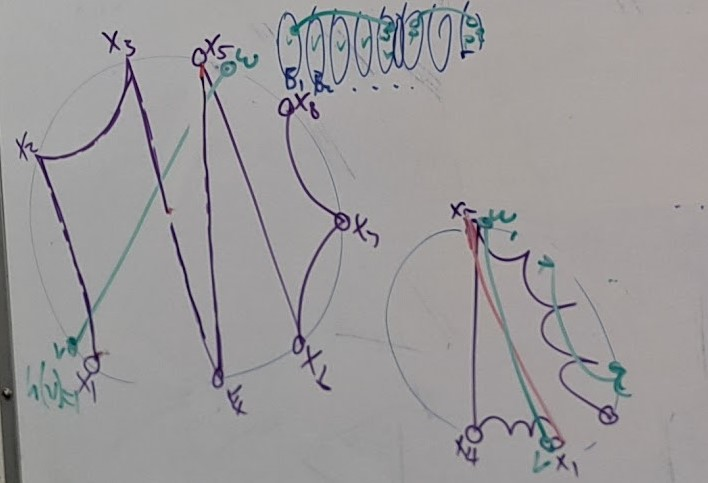
\includegraphics[width= 0.8 \textwidth]{chapters/figures/20240508_173516}
	\caption{Description of proof above. $x_1, ..., x_n$ are the vertices with a path that is a single book-embedding and $B_1, ..., B_n$ are the bags of the embedding. Notice that there are two different ways that the $n + 1$-th bag can end up, but both ways stil maintain the property that this is a book-embedding. This diagram is a circular ordering of $x_1, ..., x_n$ as it is more compact to draw.}
	\label{fig:20240508173516}
\end{figure}

\todo{Recreate diagram in tikz}

We shall now prove the lemma above.
\begin{proof}[Book-embedding lemma]
	We use the path-decomposition on $G'$ as the set $(B_1, \cdot , B_n)$ in proving this lemma. We apply the lemma above for the monochromatic $v_i$ to each of the monochromatic paths. From the construction of the vortices in \cref{lem:preserved_faces_pagenumber}, we add on the faces in the exact order. Then we have that the monochromatic paths are preserved in the ordering. 
\end{proof}

However, the issue that we run into is that the number of times each face changes colour is bounded. Let $F$ be a face and suppose the edges are in some decomposition. We define a \textit{transition point} to be a point where, when traversing a face, we change colours. We wish to devise a systems such that every face we are dealing with has a bounded number of paths.

\subsection{Planar graphs}

We have a result for planar Hamiltonian graphs, that gets us partially where we need to be. 
\begin{theorem}
	Let $G$ be a planar graph. Then every Hamiltonian cycle in $G$ preserves all faces. 
\end{theorem}

\begin{proof}
	Let $C$ be the Hamiltonian cycle of $G$. Let $D$ be the natural circular ordering of these vertices by traversing $C$. Now as $G$ is planar, $C$ splits the surface into an interior region and an exterior region, by the Jordan curve theorem. So every face is inside either the interior or exterior of $C$. But this means that every face must be preserved in $D$, as the surface we are dealing with is orientable and we can affix an orientation to every face $F$ such that the order of the vertices in the orientation is the same order as the orientation in $D$. Thus every face in this embedding is preserved. 
	\input{"chapters/figures/4-connected-planar-graph-with-cycle"}
	\todo{Make this image look like a Hamiltonian cycle in a planar graph.}
\end{proof}
As a consequence, we have that every 4-connected planar graph has a circular ordering which preserves every face. 
\subsection{Graphs on surfaces}
We first do the planar-nonplanar decomposition of $G$ first. 
Then we look at the planar subgraph $G_p$ and decompose $G_p$ into 4-connected components with adhesion at most 3, from \cref{corr:planar_graphs_4_connected_cliqesums}. 
From Tutte's theorem on planar graphs \cite{tutteTheoremPlanarGraphs1956}, we have that if $G$ is a 4-connected planar graph, then the vertex ordering of the Hamiltonian cycle $(\leq)$ preserves all faces on $G$.
In Hickingbotham's proof \cref{ssec:Clique_sum_Pagenumber_bound}, we have to move three vertices to the start of the decomposition. This will be a problem, but we claim that for every distinguished face $F$ which touches these vertices, the number of pages needed to embed $F$ is bounded. 
\todo{Add proof for this part!}

\section{Orientable surfaces}
In this section, we discuss orientable surfaces and a method for dealing with faces on an orientable surface. The non-orientable case has not been dealt with yet. 
\subsection{Non-planar decomposition}
Suppose we have a graph $G$ embedded on a surface. We apply Heath and Istrail's planar-nonplanar decomposition \cite{heathPagenumberGenusGraphs1992} to break up the edges of $G$ into $E_p$ and $E_n$, edges that are planar and nonplanar. If $F$ is bounded by planar edges, then we have that we can add a vortex to $F$ with a bounded number of pages. If $F$ is bounded by some non-planar edges, then we need additional lemmas.
We wish to show this statement:
\begin{theorem}
	For all graphs $G$ of orientable genus $g$, for all faces $F_1, ..., F_k$ of $G$, there exists a $f(g, k)$-page book embedding such that $F_i$ has $\leq h(g, k)$ monochromatic paths.
\end{theorem}

Consider $E_n$, the edges not in the planar decomposition. Consider $F_n$, the faces $F$ such that there exists an edge $e$ in $E_n$ which bounds $F$. Then we claim that the number of edges that bound $F$ is bounded. We first need an auxillary topological conjecture. We say a loop is \textit{trivial} if it is homotopy equivalent to a constant loop, and \textit{nontrivial} if this is not the case. A \textit{facial walk} is a sequence of edges $e_1, ..., e_n$ that bound a face such that $e_i$ is incident to $e_{i + 1}$ modulo $n$ for all $i$. The length of the facial walk is $n$. 

\begin{lemma}
	Let $\Sigma$ be a surface of Euler genus $g$ and let $x_0$ be a point on the surface. Then let $L$ be nontrivial loops that start and end at $x_0$ on $\Sigma$. Then let $F_1, ..., F_j$ be faces on $\Sigma + L$, such that each $F_i$ is homeomorphic to a disk. Then the length of the facial walk for all $F$ is at most $2g$. 
\end{lemma}

Parts of the proof was motivated by a discussion with Corbin Reid. The proof given is a topological one. 

\begin{proof}
	Let $G'$ be the dual graph of this graph, where the vertex set is $F_1, ..., F_j$ and the edge set are the loops, where two faces are incident if there is a loop that is touching both faces. Then take a spanning tree $T$ of $G'$, and let $L'$ be the loops that are not in $T$ and $L''$ be the loops that are in $T$. 
	Then consider embedding $L'$ on the surface $\Sigma$. Now this bounds a disk, call it $F_0$. This is a disk as we glue together $F_1, ..., F_j$ according to the spanning tree $T$, meaning that we maintain the property that the surface is contractible.
	Now we have that there is one vertex, $|L'|$ edges, and one face $F_0$. Then by Euler's formula, we have that:
	\begin{equation}
		n - m + f = 2 - g
	\end{equation}
	therefore, we have that $1 - |L'| + 1 = 2 - g$, or that $|L'| = g$. As every edge is traversed twice on either side on the facial walk, we have that the length of the facial walk is $2g$. 
	Now let us add each edge from $L''$, one at a time. We shall show that every face after adding all edges from $L''$ to $L'$ has a facial walk length of $\leq 2g$. 
	
	Before adding any edge, we have $F_0$ has $\leq 2g$ on the facial walk. Now suppose we have added loops $\gamma_1, ..., \gamma_{i - 1}$, and suppose every face has a facial walk length of $\leq 2g$. 
	Then suppose loop $\gamma_i$ splits face $F$ into faces $H$ and $J$. We have that the facial walk length $|H|$ and $|J|$ are at least 2, but bounded above by the facial walk length $F + 2$. Then we have that: 
	\begin{equation}
		2 + |J| \leq |H| + |J| \leq |F| + 2 \leq 2g + 2
	\end{equation}
	so $|J| \leq 2g$ and by symmetry so does $|H|$. Thus shown.
\end{proof}

\begin{corollary}
	Let $G$ be a graph embedded on an orientable surface $\Sigma$ with a planar-nonplanar decomposition and let $F$ be a nonplanar face. Suppose $G$ has genus $g$. Then we have that $F$ has $\leq f(g)$ monochromatic paths.
\end{corollary}

\begin{proof}
	Contract $G$ to a point. Then $F$ has at most $2g$ edges on its surface, from above. 
	Then every nonplanar face alternates between having a planar trace and nonplanar edge at most $4g$ times. Therefore, the number of monochromatic paths is bounded.
\end{proof}

By the theorem above, then we have that the planar-nonplanar decomposition has a bounded number of pages. Therefore, we are done for orientable surfaces. 